\section[Witnessing metrologically useful entanglement]
{Witnessing metrologically useful {\color{grey} X} entanglement}
\label{sec:lt}
\thiswatermark{\put(1,-282){\color{l-grey}\rule{84pt}{88pt}}
\put(84,-282){\color{grey}\rule{410pt}{88pt}}}


\quotes{Adrien-Marie Legendre}{All the truths of mathematics are linked to each other,

and all means of discovering them are equally admissible.}

\lettrine[lines=2, findent=3pt,nindent=0pt]{T}{ypically}, one has no access to the density matrix of the system which is used for metrology or for some other quantum information processing task.
Moreover, for systems in which the particle number is very large, which is the case when one wants to do metrology with quantum states, the details of the density matrix cannot be known due to practical reasons.
Since the quantum Fisher information is based on the complete knowledge of the density matrix, methods to avoid the complete tomography must be developed as we have shown a practical case in the previous chapter.
In this chapter, we obtain a general procedure to get an optimal bound for the quantum Fisher information based on as many expectation values of the initial state as one is ready to measure.
Two main features are worth to mention again.
First, in general this method gives us an optimal tight bound.
Second, the bound is based on the expectation values of the initial state only, so it is not necessary to perform an evolution of the state.
This is in contrast to other approaches one can find in the literature, ours needs a significantly smaller experimental effort.

From Eq.~\eqref{eq:bg-pezze-bound}, a lower bound on the quantum Fisher information based on expectation values of the initial state is
\be
  \qfif{\rho,J_z} \geqslant \frac{\expect{J_x}^2}{\varian{J_y}}.
\ee
where the state is polarized along the $x$-axis \cite{Pezze2009}.
In the previous chapter we have also shown one of these bounds specifically designed for unpolarized Dicke states \eqref{eq:vd-unpolarized-dicke}.

The setup is described in Section~\ref{sec:bg-quantum-magnetometry} and consists of in estimating the homogeneous magnetic field strength, in this case, which points towards the $z$-axis.
Therefore, we will base our calculations on the quantum Fisher information $\qfif{\rho, J_z}$, defined in Eqs.~\eqref{eq:bg-qfi-definition-eigen-decomposition} and \eqref{eq:bg-qfi-definition-convex-roof}, see Section~\ref{sec:bg-qfi} for more information about the properties of the QFI.

\subsection{Lower bound on a convex function given some arbitrary expectation values}

Our problem could be solved with Lagrange multipliers or Legendre transforms.
We follow the method based on Legendre transforms, since the problem of getting a lower bound of a convex function on the states having already some expectation values of some arbitrary observables has already been studied by O. G\"uhne {\it et al.} and J. Eisert {\it et al.} in Refs.~\cite{Guehne2007, Eisert2007} respectively, mainly from the perspective of entanglement measures.
The illustrated techniques are based on the well known Legendre transform for differentiable functions, see Appendix~\ref{app:legendre-transform} for more details.
We first review in this section the state-of-the-art solution to this problem.
And later on, we extend it to the quantum Fisher information.
For simplicity in the next section, Section~\ref{sec:lt-transform-for-single-observable}, we assume that a single expectation value is given.
An extension to the case in which more expectation values are given will follow in the Section~\ref{sec:lt-transform-for-m-observables}.
Finally, we will summarize our results with an explicit formula which will be used to compute the bounds in the most general case.

\subsubsection{Estimation of a general convex function based on the expectation value of an arbitrary observable}
\label{sec:lt-transform-for-single-observable}

When a convex function $g(\rho)$ is given together with an expectation value of some operator $w=\tr(\rho W)$, a tight lower bound, $\bound{g}(w)$, can be obtained as \cite{Rockafellar1996, Guehne2007, Eisert2007}
\be
  \label{eq:lt-lower-bound-single-parameter}
  \begin{split}
    g(\rho)\geqslant\bound{g}(w):=\,&\sup_r \{ rw - \hat{g}(rW)\}\\
    =\,& \{\inf_{\rho}g(\rho)\,|\,w = \tr(\rho W)\},
  \end{split}
\ee
where $\hat{g}(rW)$ is the Legendre transform of $g(\rho)$ and the second equality expresses the tightness of the bound.
The Legendre transform in this context is defined as
\be
  \label{eq:lt-for-convex-function-single-parameter}
  \hat{g}(rW)=\sup_{\rho}\{\expect{rW}_\rho - g(\rho)\},
\ee
where the maximization is over \emph{all} possible states.
This method to obtain the lower bound has been used to compute entanglement measures \cite{Guehne2007, Eisert2007}.

Following the theory one can find that in the case in which the convex function $g(\rho)$ is defined as a convex roof over all possible convex decompositions of the state, the optimisation of Eq.~\eqref{eq:lt-for-convex-function-single-parameter} can be reduced to an optimization over pure states only, thus simplifying the calculation \cite{Guehne2007, Eisert2007}
\be
\begin{split}
  \hat{g}(rW) & = \sup_{\rho}\{\expect{rW}_\rho - g(\rho)\} \\
  &=\sup_{\rho}\Big\{r\expect{W}_\rho - \inf_{\{p_k,\ket{\phi_k}\}}\big\{\sum_{k} p_k g(\ket{\phi_k})\big\} \Big\} \\
  &=\sup_{\{p_k, \ket{\phi_k}\}} \Big\{ \sum_k p_k \expect{rW}_{\ket{\phi_k}} - \inf_{\{p_k, \ket{\phi_k}\}} \big\{\sum_k p_k g(\ket{\phi_k}) \big\}  \Big\} \\
  &=\sup_{\{p_k, \ket{\phi_k}\}} \Big\{ \sum_k p_k \big\{ \expect{rW}_{\ket{\phi_k}} - g(\ket{\phi_k}) \big\} \Big\} \\
  &=\sup_{\ket{\psi}} \big\{ \expect{rW}_{\ket{\psi}} - g(\ket{\psi}) \big\}.
\end{split}
\ee
However, even an optimization over all pure states is feasible numerically only for small systems.
We will show later in this section how to circumvent this problem in the case of the QFI.
The convex roof construction has the following form
\be
  g(\rho) = \inf_{\{p_k,\psi_k\}} \sum_{k}p_k g(\ket{\psi_k}),
\ee
where the mixed state is decomposed into $\rho = \sum_k p_k \ketbra{\psi_k}{\psi_k}$.
Among other definitions of the QFI in the literature, there is one that defines it as the convex roof of $4\varian{J_z}$, the variance of the generator, as it has been shown on Ref.~\cite{Toth2007, Yu2013}, we can compute the Legendre transform optimizing for pure states only.
Hence, we will be able to use this simplification to apply this method to obtain the lower bound on the QFI.
Note that in this context, the QFI is the convex roof of four times the variance of the generator, Eq.~\eqref{eq:bg-qfi-definition-convex-roof}.

\subsubsection{Measuring several observables}
\label{sec:lt-transform-for-m-observables}

For some cases, it is interesting to characterize the quantum state not only with a single measurement but with several.
For instance, we might want to use, as it is done with the spin-squeezed states the absolute polarization and the variance of one of the orthogonal components of the angular momentum to detect entanglement and metrological usefulness \cite{Pezze2009}.
So far, we studied the case in which a single measurement is used.
Its extension to several expectation values is indeed straight-forward.
We can generalize Eqs.~\eqref{eq:lt-lower-bound-single-parameter} and \eqref{eq:lt-for-convex-function-single-parameter} for several observables $\{W_i\}_{i=1}^M$ as follows \cite{Guehne2007}
\be
  \label{eq:lt-extension-bound-multiparameter}
  \bound{g}(w_1,w_2,\dots) := \sup_{\bs{r}}\big\{\bs{rw}-\sup_{\rho}\{\expect{\bs{rW}}-g(\rho)\}\big\},
\ee
where $\bs{ab} =\sum_{k=1}^M a_kb_k$, the usual notation for scalar products of two vectors.

\subsubsection{Explicit form of the expression to be optimized}

After we have shown how to find a lower bound for a general convex function of the state based on its expectation values and how to simplify that method for the case in which the function is defined as a convex roof, now we are in the position to achieve the main goal of this chapter.
First of all, we note that for the quantum Fisher Information the inner maximization, the Legendre transform, is obtained optimizing a function quadratic in expectation values,
\be
\label{eq:lt-legendre-of-qfi}
\begin{split}
  \hat{\qfi}(rW) &= \sup_{\ket{\psi}}\big\{r\expect{W}_{\psi}-4\varian{J_z}_{\psi}\big\} \\
  &= \sup_{\ket{\psi}} \big\{ r\expect{W}_{\psi}-4\expect{J_z^2}_{\psi} + 4\expect{J_z}^2_{\psi} \big\} \\
  &= \sup_{\ket{\psi}} \big\{\expect{rW-4J_z^2}_{\psi} +
  \expect{2J_z}^2_{\psi}\big\},
\end{split}
\ee
where we have used the fact that the QFI can be expressed as a convex roof of $\varian{J_z}$ and we arrive at the problem of an optimization over a single parameter for simplicity on the following derivations.
Equation~\eqref{eq:lt-legendre-of-qfi} can be rewritten as an optimization linear in operator expectation values and over a parameter $\mu$ as
\be
  \hat{\mathcal{F}}_{\text{Q}}(rW) = \sup_{\ket{\psi},\mu}\big\{\expect{rW-4J_z^2}_{\psi}+8\mu\expect{J_z}_\psi - 4 \mu^2\mtxid\big\},
\ee
which, making use of $\max\{\expect{A}\}=\lambda_{\max}[A]$ for any observable, can be reformulated as
\be
  \label{eq:lt-legendre-for-qfi-simplified}
  \begin{split}
    \hat{\mathcal{F}}_{\text{Q}}(rW) & = \sup_{\ket{\psi}}\big\{\lambda_{\max}[rW-4J_z^2+8\mu J_z - 4 \mu^2]\big\}\\
    &=\sup_{\ket{\psi}}\big\{\lambda_{\max}[rW-4(J_z-\mu)^2]\big\},
  \end{split}
\ee
where we omitted in writing $\mtxid$ for clarity and $\lambda_{\max}[A]$ stands for the maximum eigenvalue of the operator $A$.
At the extremum, the derivative with respect to $\mu$ must be zero, hence at the optimum $\mu=\expect{J_z}_{\text{opt}}$ which represents the expectation value of $J_z$ should have considering the optimal state in Eq.~\eqref{eq:lt-legendre-of-qfi}.
This also means that we have to test $\mu$ values in the interval $-N/2\leqslant\mu\leqslant N/2$ only for spin-half systems.

The full optimization problem to be solved consists of Eqs.~\eqref{eq:lt-lower-bound-single-parameter} and~\eqref{eq:lt-legendre-for-qfi-simplified} substituting $g(\rho)$ by $\qfif{\rho,J_z}$,
\be
  \bound{\mathcal{F}}(w) = \sup_r\big\{rw-\sup_{\mu}\{\lambda_{\max}[rW-4(J_z-\mu)^2]\}\big\}.
  \label{eq:lt-bound-for-qfi}
\ee
It is crucial that the optimization over $r$ is a concave function, since the theory tells us that $\hat{\mathcal{F}}_{\text{Q}}(rW)$ is a convex function \cite{Rockafellar1996}, even when the multi-parameter case is considered.
Thus the optimum can be determined easily with simple methods, e.g., the gradient method, looking for the maximum in $r$.
Based on Eq.~\eqref{eq:lt-lower-bound-single-parameter}, we can see that even if we do not find the global optimum in $r$, we obtain a valid lower bound.
The extension of this bound to the multi-parameter case is done using the recipe given in Eq.~\eqref{eq:lt-extension-bound-multiparameter}.
On the other hand, the function to be optimized for $\mu$ does not have a single maximum in general.
Moreover, not finding the optimal $\mu$ leads to an overestimating of the bound.
Thus, a large care must be taken when optimizing over $\mu$.

We stress again the generality of these findings beyond linear interferometers covered on the following sections.
For nonlinear interferometers \cite{Luis2004, Boixo2007, Choi2008, Roy2008, Napolitano2011, Hall2012}, the phase $\theta$ must be estimated assuming unitary dynamics $U=\exp{-iG\theta}$, where $G$ is not a sum of single spin operators, hence, it is different from the angular momentum components.

Next, we will demonstrate the use of our approach for several experimentally relevant situations.
In the many-particle case, often symmetric operators can be used to describe accurately the system, which makes it possible to carry out calculations for thousand of particles, as will be presented later in this chapter.

\subsection{Examples}
\label{sec:lt-examples}

In this section, we show how to obtain lower bounds based on the fidelities with respect to the GHZ state and the unpolarized Dicke state as well as with different set of powers of collective angular momentum operators, e.g., the set $\{\expect{J_y}, \expect{J_x}, \expect{J_x^2}\}$.

\subsubsection{Exploiting symmetries}
\label{sec:lt-symmetries}

When making calculations for quantum systems with an increasing number of qubits, we soon run into difficulties when computing the largest eigenvalue of Eq.~\eqref{eq:lt-legendre-for-qfi-simplified}.
The reason is that for $N$ qubits, we need to handle $2^N \times 2^N$ size matrices, hence we are limited to systems of 10 to 15 qubits.

We can obtain bounds for much larger particle numbers, if we restrict ourselves to the symmetric subspace \cite{Toth2007, Toth2009a}.
This approach can give optimal bounds for many systems, such as Bose-Einstein condensates of two-level atoms, which are in a symmetric multiparticle state.
The bound computed for the symmetric subspace might not be correct and generally might overestimate the real bound for general cases.

Finally, it is important to note that if the operators $W_k$ are permutationally invariant (PI) and the eigenstate with the maximal eigenvalue in Eq.~\eqref{eq:lt-legendre-for-qfi-simplified} is non-degenerate, then, we can do the computations on the symmetric subspace only.
The resulting maximal eigenvalue is the maximal eigenvalue when the whole Hilbert space is taken into account for the maximization.
Hence, the lower bound obtained in the symmetric subspace is valid even for the general case.

We follow presenting the proof of the recently mentioned observation for completeness.
Let us denote the ground state of a permutationally invariant Hamiltonian by $\ket{\Psi}$
This is at the same time the $T=0$ thermal ground state, hence it must be a permutationally invariant pure state.
For such states $S_{kl}\ketbra{\Psi}{\Psi}S_{kl}=\ketbra{\Psi}{\Psi}$, where $S_{kl}$ is the swap operator exchanging qubits $k$ and $l$.
Based on this, follows that $S_{kl}\ket{\Psi}=c_{kl}\ket{\Psi}$, and $c_{kl}\in {-1,+1}$.
There are three possible cases to consider:
\begin{enumerate}
  \item All $c_{kl}=+1$.
  In this case, for all permutation operator $\Pi_j$ we have
  \be
    \label{eq:lt-permutating-ground-state}
    \Pi_j \ket{\Psi} = \ket{\Psi},
  \ee
  since any permutation operator $\Pi_j$ can be constructed as $\Pi_j=\prod_i S_{k_il_i}$.
  Equation~\eqref{eq:lt-permutating-ground-state} means that the state $\ket{\Psi}$ is symmetric.
  \item All $c_{kl}=-1$.
  This means that the state is anti-symmetric, however this state exists only for $N=2$ qubits.
  \item Not all $c_{kl}$ are identical to each other.
  In this case, there must be $k_+,l_+,k_-,k_-$ such that
  \be
    \label{eq:lt-different-index-pi}
    \begin{split}
      S_{k_+,l_+} \ket{\Psi} & = +\ket{\Psi},\\
      S_{k_-,l_-} \ket{\Psi} & = -\ket{\Psi}.
    \end{split}
  \ee
  Let us assume that $k_+,l_+,k_-,l_-$ are index different from each other.
  In this case, $\ket{\Psi'}=S_{k_+,k_-}S_{l_+,l_-}\ket{\Psi}$ another ground state of the Hamiltonian $H$ such that
  \be
    \label{eq:lt-different-index-pi-2}
    \begin{split}
      S_{k_+,l_+} \ket{\Psi'} & = -\ket{\Psi'},\\
      S_{k_-,l_-} \ket{\Psi'} & = +\ket{\Psi'}.
    \end{split}
  \ee
  Comparing Eqs.~\eqref{eq:lt-different-index-pi} and \eqref{eq:lt-different-index-pi-2} we can conclude that $\ket{\Psi'}\neq\ket{\Psi}$, while due to the permutational invariance of $H$ we have that $\expect{H}_{\Psi'} = \expect{H}_{\Psi}$.
  Thus, $\ket{\Psi}$ is not a non-degenerate ground state.
  The proof works in an analogous way for the only nontrivial case $k_+=k_-$, when $S_{k_+,k_-}=\mtxid$.
\end{enumerate}

Hence, if $N>2$ then only i) is possible and $\ket{\Psi}$ must be symmetric.

\subsubsection{Fidelity measurements}
\label{sec:lt-bounds-fidelity}

Let us consider the case when $W$ is a projector onto a pure quantum state.
First, we consider GHZ states.
Hence $W$ is the projector $\ketbra{\ghz}{\ghz}$, where
\be
  \ket{\ghz} = \tfrac{1}{\sqrt{2}}(\ket{0\cdots0}+\ket{1\cdots1})
  \label{eq:lt-ghz-state}
\ee
for spin-$\frac{1}{2}$ particles, and $\expect{W}=F_{\ghz}$ is the fidelity with respect to the GHZ state.
Based on knowing $F_{\ghz}$, we would like to estimate $\qfif{\rho,J_z}$\footnote{
Not a tight lower bounds on the quantum Fisher information based on the fidelity have been presented in \cite{Augusiak2016}.}.

Using Eq.~\eqref{eq:lt-bound-for-qfi}, we will obtain an analytical tight lower bound on the QFI based on the fidelity $F_{\ghz}$. The calculation that we have to carry out is computing the bound
\be
  \label{eq:lt-maximization-problem-fid-ghz}
  \bound{\mathcal{F}}(F_{\ghz}) = \sup_r \big\{r F_{\ghz} - \sup_{\mu} \{\lambda_{\max}[r\ketbra{\ghz}{\ghz} - 4 (J_z - \mu)^2]\}\big\}.
\ee
We will make our calculations in the $J_z$ orthonormal basis, which is defined with the $2^N$ basis vectors $b_0= \ket{00\dots000}$, $b_1=\ket{00\dots001}$, \dots, $b_{(2^N-2)}=\ket{11\dots110}$, and $b_{(2^N-1)}=\ket{11\dots111}$, as it can be found in Eq.~\eqref{eq:app-eigenbasis-tensor-product} for $j=\frac{1}{2}$.
It is easy to see that the matrix in the argument of $\lambda_{\max}$ in the Eq.~\eqref{eq:lt-maximization-problem-fid-ghz} is almost diagonal in the $J_z$ basis.
To be more specific, the only non-diagonal matrix block comes from $\ketbra{\ghz}{\ghz}$, which has non-trivial matrix elements only in the $\{b_0,b_{(2^N-1)}\}$ basis.
Thus, we have to diagonalize the following matrix
\be
  \label{eq:lt-expression-to-diagonalize-ghz}
  r\ketbra{\ghz}{\ghz} - 4 (J_z-\mu)^2 =
  \begin{pmatrix}
    \frac{r}{2}-4(\frac{N}{2}-\mu)^2 & \frac{r}{2}\\
    \frac{r}{2} & \frac{r}{2}-4(\frac{N}{2}+\mu)^2
  \end{pmatrix}
  \oplus D,
\ee
where $D$ is already a $(2^N-2)\times(2^N-2)$ diagonal matrix with $D_k=-4( \expect{J_z}_{b_k}-\mu)^2$ negative eigenvalues for $k=1,2,\dots, (2^N-2)$.
This means that the Eq.~\eqref{eq:lt-expression-to-diagonalize-ghz} can be diagonalized as $\text{diag}[\lambda_{+},\lambda_{-},D_1,D_2,\dots,D_{2^N-2}]$, where the two eigenvalues $\lambda_{\pm}$ are
\be
  \lambda_{\pm} = \frac{r}{2}-N^2-4 \mu^2\pm\sqrt{16\mu^2N^2+\frac{r^2}{4}}.
\ee

Next, we show a way that can simplify our calculations considerably.
As indicated in Eq.~\eqref{eq:lt-maximization-problem-fid-ghz}, we have to look for the maximal eigenvalue and then optimize it over $\mu$.
We exchange the order of the two steps, that is, we look for the maximum of each eigenvalue over $\mu$, and then find the maximal one.
Clearly based on the fact that the eigenvalues of $D$ are negative an that we can find a $\mu$ such that $D_k$ equal zero but not positive.
Due to this, the problem can be simplified to the following equation
\be
  \label{eq:lt-ghz-legendre-solution}
  \begin{split}
  \sup_{\mu}\{\lambda_{\max}[r\ketbra{\ghz}{\ghz}-4(J_z-\mu)^2]\}:= & \max\{0,\sup_{\mu}(\lambda_{+})\}\\
  = & \lcor
  \begin{aligned}
    &0, && \text{if } r<0,\\
    &\frac{r}{2}+\frac{r^2}{16N^2} && \text{if } 0\leqslant r\leqslant 4N^2,\\
    &-N^2+r, && \text{if }r>4N^2,
  \end{aligned}
  \right.
  \end{split}
\ee
where we did not have to have to look for the maximum of $\lambda_{-}$ over $\mu$ since clearly $\lambda_{+}\geqslant\lambda_{-}$.
Finally, we have to substitute Eq.~\eqref{eq:lt-ghz-legendre-solution} into Eq.~\eqref{eq:lt-maximization-problem-fid-ghz}, and carry out the optimization over $r$, considering $F_{\ghz}\in[0,1]$.

This way we arrive at the solution for the lower bound of the QFI base on the fidelity with respect to the GHZ state as
\be
  \bound{\mathcal{F}}(F_{\ghz}) = \lcor
  \begin{aligned}
    & N^2(1-F_{\ghz})^2, && \text{if } F_{\ghz} < 1/2, \\
    & 0, && \text{if } F_{\ghz}\leqslant1/2.
  \end{aligned}
  \right.
\ee
This equation is plotted in Figure~\ref{fig:lt-plots-for-fidelities}.a.
Note that in the figure the plot is normalized by $N^2$ and that the resulting semi-parabola is independent of the number of particles.
Moreover, the bound is zero for $F_{\ghz}\leqslant 1/2$.
This is consistent with the fact that for the product states $\rho=\ket{111\dots11}$ or $\rho=\ket{000\dots00}$ we have $F_{\ghz}=1/2$, while $\mathcal{F}_{\text{Q}}[\rho,J_z]=0$.
\begin{figure}[htp]
  \centering
  \igwithlabel{(a)}{scale=.65}{img/LT_fidGHZ.pdf}
  \igwithlabel{(b)}{scale=.65}{img/LT_fidDicke.pdf}
  \caption[Lower bound for fidelities. (a) $F_{\text{GHZ}}$. (b) $F_{\text{Dicke}}$.]{(a) Analytical solution of the bound $\bound{\mathcal{F}}$ for different values of the fidelity with respect to the GHZ state.
  (b) Numerical results for the minimum quantum Fisher information as a function of the fidelity with respect of unpolarized Dicke states perpendicular to the magnetic field, $|\text{D}_N^0\rangle$.
  (blue-line) For systems with 4 particles and (red-dashed) for system with 8 particles. One may note that when the fidelity is at its maximum the bound approaches to 0.5 as it is the quantum Fisher information for large particle number.}
  \label{fig:lt-plots-for-fidelities}
\end{figure}

Next, let us consider a symmetric unpolarized Dicke state with even $N$ particles along the $x$-direction $\ket{\dicke{N}}_x$, given by Eq.~\eqref{eq:vd-unpolarized-dicke}.
This state is known to be highly entangled \cite{Toth2007, Toth2009} and allows for a Heisenberg limited interferometry \cite{Holland1993}.
In the following we may omit the subscript $x$ since this Dicke state will be always at the center of our attention, the unpolarized Dicke state perpendicular to the magnetic field in this case along the $z$-direction.
The witness operator that can be used for noisy Dicke states is $W=\ketbra{\dicke{N}}{\dicke{N}}$, hence the expectation value of the witness is just the fidelity with respect to the Dicke state, i.e., $\expect{W}=F_{\text{Dicke}}$.
In Figure~\ref{fig:lt-plots-for-fidelities}.b, we plotted the results for symmetric Dicke states of various spin numbers.
$F_{\text{Dicke}}=1$ corresponds to $\mathcal{F}_{\text{Q}}[\rho,J_z]=N(N+2)/2$.
At this point, note that for the examples presented above, the QFI bound scales as $\mathcal{O}(N^2)$ in the asymptotic limit if the quantum state has been prepared perfectly\footnote{$\mathcal{O}(x)$ is the usual Landau notation used to describe the asymptotic behavior for large $x$ \cite{Hyllus2012, Toth2012}.}.

Note that estimating $\qfif{\rho, J_z}$ based on $F_{\text{Dicke}}$ was possible for 40 qubits [TD: Ask geza for the data points for 40 particles] for Fig~\ref{fig:lt-plots-for-fidelities}.b, since we carried out the calculations for the symmetric subspace.
For our case, the witness operator $W$ is permutationally invariant and it has a non-degenerate eigenstate corresponding to the maximal eigenvalue.
Hence, based on the arguments of the Section~\ref{sec:lt-symmetries} the bound is valid even for the general case, i.e., non-symmetric states.

We now compute several quantities for the large $N$ case.
We show that if the fidelity with respect to the Dicke state is larger than a bound then $\bound{\mathcal{F}}>0$, where we omit the arguments for brevity.
Moreover, we have seen in Figure~\ref{fig:lt-plots-for-fidelities}.b that the lower bound on $\qfif{\rho,J_z}$ as a function of the fidelity $F_{\text{Dicke}}$ normalized by $N^2$ is not the same curve for all $N$.
Next, we will demonstrate by numerical evidence that the lower bound normalized by $N^2$ collapses to a nontrivial curve for large $N$.

As a first step, let us consider the state completely polarized along $z$-direction $\ket{1}_y^{\otimes N}$.
This state does not change under rotations around the $z$-axis, hence $\qfif{\rho,J_z}=0$.
Its fidelity with respect to the Dicke state $\ket{\dicke{N}}_x$ is
\be
  \label{eq:lt-fidelity-dicke-with-tp}
  F_{\text{Dicke}}(\ket{1}_y^{\otimes N}) = \frac{1}{2^N}\binom{N}{N/2}\approx \sqrt{\frac{2}{\pi N}}
\ee
From convexity of the bound on the quantum Fisher information in $F_{\text{Dicke}}$, it immediately follows that for $F_{\text{Dicke}}$ smaller than Eq.~\eqref{eq:lt-fidelity-dicke-with-tp} the optimal bound on $\qfif{\rho,J_z}$ will give zero.

Next, we examine what happens if the fidelity is larger than Eq.~\eqref{eq:lt-fidelity-dicke-with-tp}.
For that we note first that $\qfif{\rho,J_z}$ is the convex roof of $4\varian{J_z}$ \cite{Toth2013, Yu2013}.
Hence, if we have a mixed state for which $\qfif{\rho,J_z}$ is zero, then it can always be decomposed into the mixture of pure states for which $\qfif{\ket{\Psi},J_z}$ is zero too.
As a consequence, the extremal states of the set of states for which $\qfif{\rho,J_z}=0$ are pure states, and we can restrict our search for pure states.
The optimization problem we have to solve is given as
\be
  F_{\text{opt}} = \big\{ \max_{\Psi} |\braket{\Psi}{\dicke{N}}_x|^2 \,|\, \qfif{\ket{\Psi},J_z}=0\big\}.
\ee
Pure states $\ket{\Psi}$ that are invariant under $U_{\theta}=\exp(-iJ_z\theta)$ for any $\theta$.
Such states are the eigenstates of $J_z$.
In order to maximize the overlap with the Dicke state $\ket{\dicke{N}}_{x}$, we have to look for symmetric eigenstates of $J_z$.
These are the symmetric Dicke states in the $z$-basis $\ket{\dicke{N,m}}_z$.
Then, using the following identity
\be
  \sum_{k=0}^q (-1)^k \binom{n}{k}\binom{n}{q-k} = \lcor
  \begin{aligned}
    &\binom{n}{q/2}(-1)^{q/2},&& \text{for even }q,\\
    &0, && \text{for odd }q.
  \end{aligned}
  \right.
  \label{eq:lt-binomial-identity}
\ee
one finds that the squared overlap is given by
\be
  |\braopket{\dicke{N,m}}{_z}{\dicke{N}}_x|^2 = \lcor
  \begin{aligned}
    &\frac{\binom{N/2}{m/2}^2\binom{N}{N/2}}{2^N\binom{N}{m}} ,&& \text{for even }m \text{ and }N,\\
    &0, && \text{for odd }m,
  \end{aligned}
  \right.
  \label{eq:lt-dicke-overlap}
\ee
which is maximal, in the case of even $N$, when $m=N$ or $m=0$, thus the state totally polarized along $+z$-direction or $-z$-direction respectively.
We skip the case in which $N$ is odd.
For detailed calculations of Eq.~\eqref{eq:lt-dicke-overlap} see Appendix~\ref{app:calculation-dicke-overlap}.

Next, we will examine the behavior of our lower bound on $\qfif{\rho,J_z}$ based on the fidelity $F_{\text{Dicke}}$ for large $N$.
In Figure~\ref{} [TD: Ask Geza for the data], the calculations up to $N=500$ present a strong evidence that for fidelity values $F_{\text{Dicke}}=0.2,0.5,0.8$ the lower bound on QFI has a $\mathcal{O}(N^2)$ scaling for increasing $N$.
If this is correct then reaching a fidelity larger than a certain monotonously decreasing bound for large $N$ would imply Heisenberg scaling for the bound on the quantum Fisher information.
Note that it is difficult to present a similar numerical evidence for small values of $F_{\text{Dicke}}$ since in that case the bound for QFI is nonzero only for large $N$ due to Eq.~\eqref{eq:lt-fidelity-dicke-with-tp}.

\subsubsection{Spin-squeezed states}
\label{sec:lt-bound-spsq}

In the case of spin squeezing, the quantum state has a large spin in the $y$-direction, while a decreased variance in the $x$-direction.
By measuring $\expect{J_y}$ and $\varian{J_x}$ we can estimate the lower bound for the quantum Fisher Information by Eq.~\eqref{eq:bg-pezze-bound}.
However, this formula does not necessarily give the best lower bound for all values of the collective observables.
With our approach we can find the best bound.

To give a concrete example, we choose $W_1=J_y$, $W_2=J_x^2$ and $W_3=J_x$ for the operators to be measured.
We vary $w_1$ and $w_2$ in some interval.
We also require that $w_3=0$, since we assume that the mean spin points into the $y$-direction\footnote{
Due to symmetries of the problem, when minimizing $\qfif{\rho,J_z}$ with the constraints on $\expect{J_z}$ and $\expect{J_x^2}$, we do not have to add explicitly the constraint $\expect{J_x}=0$.
Optimization with only the first two constraints will give the same bound (see Section~\ref{sec:}).}
This is reasonable since in most spin-squeezing experiments we know the direction of the mean spin.

Our result can be seen in Figure~\ref{fig:lt-spsq2d-4}.
We chose $N=4$ particles since for small $N$ the main features of the plot are clearly visible.
The hatched area corresponds to non-physical combination of expectation values.
States at the boundary can be obtained as ground states of $H_{\text{bnd}}^{(\pm)}(\lambda)=\pm J_x^2 -\lambda J_y$, see Appendix~\ref{app:spin-squeezing-hamiltonian}.
In Figure~\ref{fig:lt-spsq2d-4}, the state fully polarized in the $y$-direction, and initial state for spin-squeezing experiments, corresponds to point T.
The unpolarized Dicke state along the $x$-direction Eq.~\eqref{eq:vd-unpolarized-dicke} corresponds to point D.
We add that outside the symmetric subspace, there are other states with $\expect{J_y}=\expect{J_x^2}=0$, which also correspond to the point D, e.g the single state labeled by the point S.
However, usual spin-squeezing procedures remain in the symmetric subspace, thus we discuss only the Dicke state.
Spin squeezing makes $\varian{J_x}$ decrease, while $\expect{J_y}$ also decreased somewhat.
Hence, at least for small squeezing it corresponds moving down from point T to point D following the boundary, while the metrological usefulness is increasing.
Below the dashed line $\qfif{\rho,J_z}>N$, hence the state possesses metrologically useful entanglement \cite{LT3}.
The equal mixture of $\ket{000\dots00}_x$ and $\ket{111\dots11}_x$ corresponds to point M, with $\qfif{\rho,J_z} = N$.
Finally, the completely mixed state rests on the line W.
It cannot be used for metrology, hence $\qfif{\rho,J_z}=0$.
\begin{figure}[htp]
  \centering
  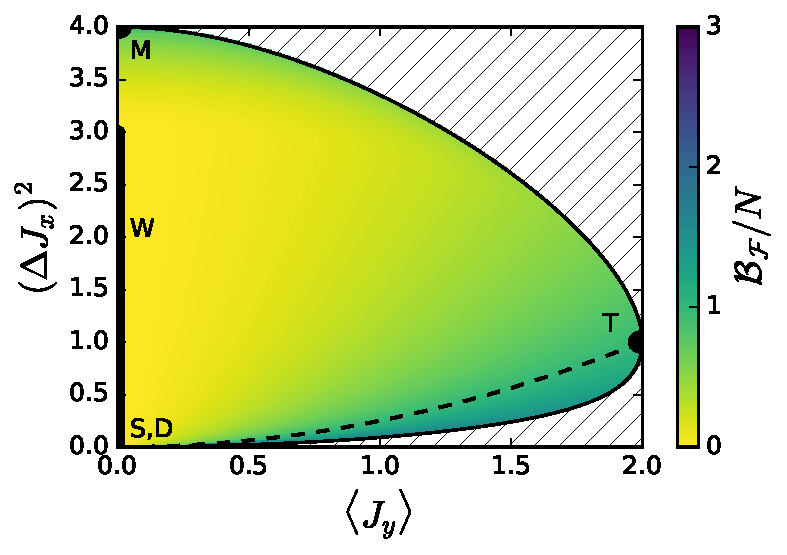
\includegraphics[scale=.65]{img/LT_spsq2d_4.pdf}
  \caption[Solution for 4 particle on the paramenter region for spin-squeezed states.]{We show as a function of the expectation value, $\expect{J_y}$, and the variance in the perpendicular direction, $\varian{J_x}$, the minimum sensitivity for a 4-qubit system.
  (hatched) The physically forbidden region is indicated. (M,T,S,D) Those points indicate where the mixed state (M), the state totally polarized (T), the singlet state (S) and the unpolarized Dicke state (D) would be located. (W) Any of the states from the completely mixed state of the symmetric subspace to the singlet state is in this line. For instance, one can  find the completely mixed state of the whole Hilbert space sitting in that line. (dashed) Shot-noise threshold. Below this line non-classical sensitivities can be achieved.}
  \label{fig:lt-spsq2d-4}
\end{figure}

We now compare the difference between our bound and the bound of L.~Pezze and A.~Smerzi Eq.~\eqref{eq:bg-pezze-bound}.
First, we consider the experimentally relevant region for which $\varian{J_x}\leqslant 1$.
We find that for points away from the physical boundary at least by 0.001 on the vertical axis, the difference between the two bounds is smaller than $2\times10^{-6}$.
Hence, Eq.~\eqref{eq:bg-pezze-bound} practically coincides with the optimal bound for $\varian{J_x}<1$.

For points at the boundary, the difference is somewhat larger, but still small, the relative difference is smaller than $2\%$ for 4 particles.
We compute the difference between the Eq~\eqref{eq:bg-pezze-bound} and our bound for different number of particles and for states at the boundary from the state totally polarized T to the unpolarized Dicke state at D, see Figure~\ref{fig:lt-edge-diff}.
\begin{figure}[htp]
  \centering
  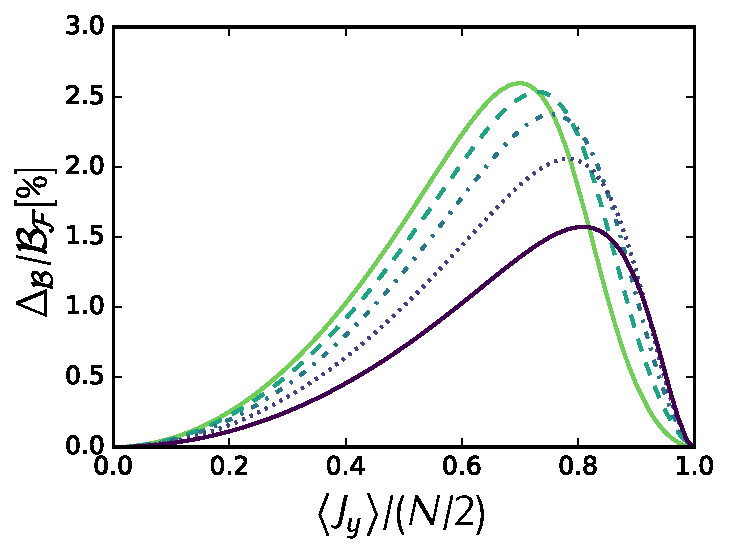
\includegraphics[scale=.65]{img/LT_edge_diff.pdf}
  \caption[Boundary difference of optimal bound versus Pezz\'e-Smerzi bound.]{Difference between the bound of Pezze-Smerzi and the optimal bound for the quantum Fisher information normalized by the value of the optimal bound itself for the bosonic ground states of $H=J_x^2-\lambda J_y$ for $\forall \lambda \in [0,\infty)$.
  From dark to lighter colors (line, point, dash-point, dashed, pointed, line), results for different particle numbers, $N=4,6,10,20,1000$ respectively.
  One can see that for large particle numbers the difference is largest when the polarization is around two thirds of the maximal polarization and that this difference is less than $2.6\%$.}
  \label{fig:lt-edge-diff}
\end{figure}

We now consider regions on Figure~\ref{fig:lt-spsq2d-4} for which $\varian{J_x}>1$.
The difference between the two bound is now larger.
It is larger at point M, for which the bound Eq.~\eqref{eq:bg-pezze-bound} is zero.
Hence for measurement values corresponding to points close to M, our method improve the formula Eq.~\eqref{eq:bg-pezze-bound}.
It is important from the point of view of applying our method to spin-squeezing experiments that the bound Eq.~\eqref{eq:bg-pezze-bound} can be substantially improved for $\varian{J_x}<1$, if we assume bosonic symmetry for the system, or we measure an additional quantity, such as $\expect{J_x^4}$ as shown in Figure~\ref{fig:lt-adding-jx4-to-the-bound} [TD: Ask Geza for data].
\begin{figure}[htp]
  \centering
  % 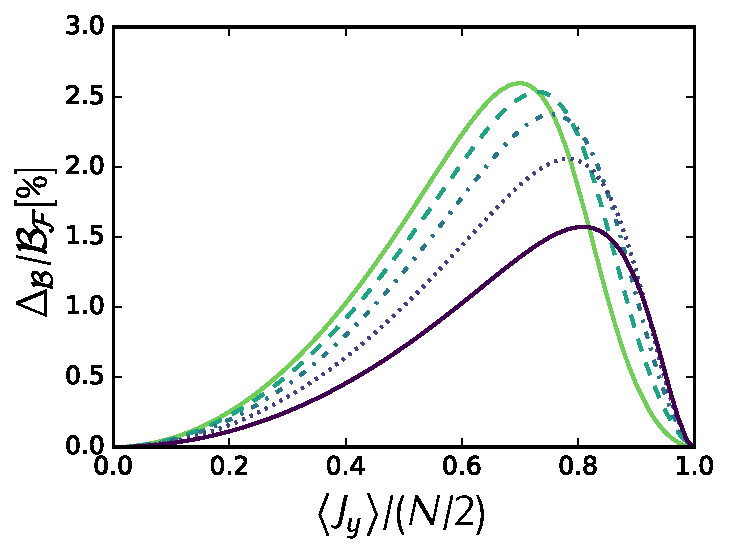
\includegraphics[scale=.65]{img/LT_edge_diff.pdf}
  % \caption[Boundary difference of optimal bound versus Pezz\'e-Smerzi bound.]{Difference between the bound of Pezze-Smerzi and the optimal bound for the quantum Fisher information normalized by the value of the optimal bound itself for the bosonic ground states of $H=J_x^2-\lambda J_y$ for $\forall \lambda \in [0,\infty)$.
  % From dark to lighter colors (line, point, dash-point, dashed, pointed, line), results for different particle numbers, $N=4,6,10,20,1000$ respectively.
  % One can see that for large particle numbers the difference is largest when the polarization is around two thirds of the maximal polarization and that this difference is less than $2.6\%$.}
  \label{fig:lt-adding-jx4-to-the-bound}
\end{figure}


\subsubsection{Dicke states}
\label{sec:lt-bound-dicke-states}

In this section, we use our method to find lower bounds on the QFI for states close to the Dicke states \eqref{eq:vd-unpolarized-dicke} along the $x$-direction, based on collective measurements.
We discuss what operators have to be measured to estimate the metrological usefulness of the state.
In Section~\ref{sec:lt-many-particle-experiments}, we will test our approach for a realistic system with very many particles.

In order to estimate the metrological usefulness of states created in such experiments, we choose to measure $W_1=J_x^2$, $W_2=J_y^2$ and $W_3=J_z^2$ since the expectation values of these operators uniquely define the ideal Dicke state, and they have been already used for entanglement detection \cite{Luecke2014}.
In cold gas experiments of nowadays, the state created is invariant under transformations of the type $U_{x}(\phi)=\exp(-i J_x \phi)$ \cite{Apellaniz2015}.
For such states $\expect{J_y^2}=\expect{J_z^2}$, which we also use as a constraint in our optimization.

Let us demonstrate how our method works in an example for small systems.
Figure~\ref{fig:lt-symmetric-dicke-6-bound}
\begin{figure}[htp]
  \centering
  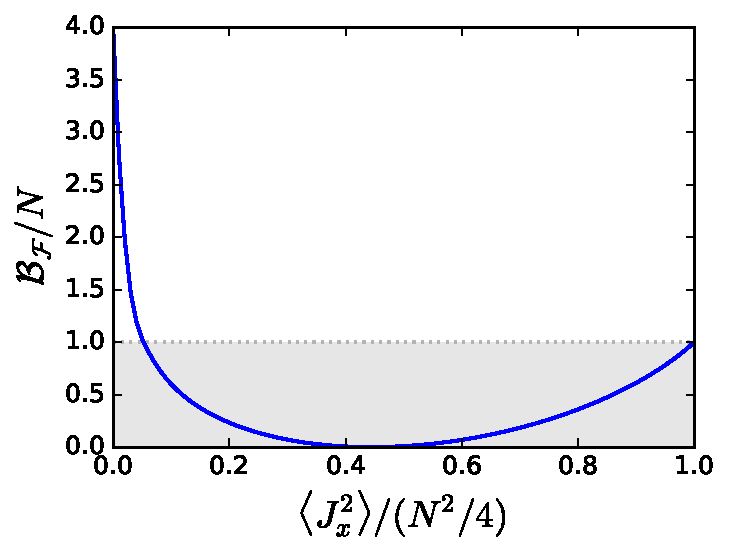
\includegraphics[scale=.65]{img/LT_dicke_edge.pdf}
  \caption[6-particles optimal bound on BEC symmetry for the QFI when $\{\expect{J_x^2},\expect{J_y^2},\expect{J_z^2}\}$ are measured]{Optimal lower bound on the quantum Fisher Information for symmetric states with $\expect{J_y^2}=\expect{J_z^2}$. Even if it is metrologicaly useful for a wide range of $\expect{J_x^2}$, the numerics shows us a tiny region where the metrological gain is surpassing the shot-noise limit.}
  \label{fig:lt-symmetric-dicke-6-bound}
\end{figure}
shows the result for 6 qubits for symmetric states for which
\be
  \label{eq:lt-maximum-angular-momentum}
  \expect{J_x^2+J_y^2+J_z^2} = \frac{N(N+2)}{4}=:\mathcal{J}_N.
\ee
It can be seen that the lower bound on quantum Fisher Information is the largest for $\expect{J_x^2}=0$.
It reaches the value corresponding to the ideal Dicke state, $\qfif{\rho,J_z}/N=(N+2)/2=4$.
It is remarcable that the state is also useful for metrology if $\expect{J_x^2}$ is very large.
In this case $\expect{J_y^2}$ and $\expect{J_z^2}$ are smaller than $\expect{J_x^2}$.

\subsection{Calculations for experimental data}

In this section, we use our method to find tight lower bound on the QFI based on experimental data.
In particular, we will determine the bound for several experiments in photons and trapped ions creating GHZ states and Dicke states, in which the fidelity has been measured \cite{Krischek2011, Zhao2003, Gao2010, Leibfried2004, Sackett2000, Monz2011, Kiesel2007, Wieczorek2009, Prevedel2009, Chiuri2012}, which is much easier than obtaining the quantum Fisher Information from the density matrix \cite{Hyllus2012}, or estimation it from a metrological procedure \cite{Luecke2011}.
We will obtain a bound on the QFI for a spin-squeezing experiment with thousand of particles \cite{Gross2010}.
Based on numerical examples, we see that the bound Eq.~\eqref{eq:bg-pezze-bound} is close to the optimal even for not completely polarized states.
Assuming symmetry or knowing additional expectation values can improve the bound Eq.~\eqref{eq:bg-pezze-bound}.
Finally, we will also obtain the bound for the QFI for a recent experiment with Dicke states \cite{Luecke2014}.
The estimate of the precision based on considering the particular case when $\expect{J_x^2}$ is measured for parameter estimation \cite{Apellaniz2015} is close to the optimal bound computed by our method.

\subsubsection{Few-particle experiments}

Now, we will estimate the quantum Fisher information based on the fidelity with respect to Dicke states and GHZ states for several experiments with photons and trapped cold ions, following the ideas of Section~\ref{sec:lt-bounds-fidelity}.

Our results are summarized in Table~\ref{tab:lt-results-for-fidelities}.
The experiments in \cite{Gao2010,Chiuri2012} are with hyperentangled qubits, while in the rest of experiments a single qubit is stored in a particle.
Ref.~\cite{Monz2011} describes experiments with 2-14 ions, we presented only results of two of them.
Finally, for the experiment of Ref.~\cite{Zhao2004} we used the fidelity estimated using reasonable assumptions discussed in that paper, while the worst case fidelity is lower.
\begin{table}
  \begin{center}
    \begin{tabular}{| l | l | l | l | l |}
      \hline
      Physical&Target &\multicolumn{1}{ l|}{\multirow{2}{*}{Fidelity}}
      &\multicolumn{1}{ l|}{\multirow{2}{*}{$\bound{\mathcal{F}}/N$}}
      &\multicolumn{1}{ l|}{\multirow{2}{*}{Ref.}} \\
      system & quantum state &  &  &  \\ \hline
      \multicolumn{1}{|l|}{\multirow{6}{*}{photons}}
      & \multicolumn{1}{ l|}{\multirow{4}{*}{$\ket{\dicke{4}}$}}
      & $0.844\pm0.008$   & $1.432\pm0.044$ & \cite{Kiesel2007} \\
      & & $0.78\pm0.008$    & $1.124\pm0.236$ & \cite{Chiuri2012} \\
      & & $0.8872\pm0.0055$ & $1.680\pm0.036$ & \cite{Krischek2011} \\
      & & $0.873\pm0.005$   & $1.44\pm0.024$  & \cite{Toth2010} \\ \cline{2-5}
      & \multicolumn{1}{ l|}{\multirow{2}{*}{$\ket{\dicke{6}}$}} &
      $0.654\pm0.024$   & $0.564\pm0.076$ & \cite{Wieczorek2009} \\
      & & $0.56\pm0.02$     & $0.304\pm0.048$ & \cite{Prevedel2009} \\ \hline
      \multicolumn{1}{|l|}{\multirow{5}{*}{photons}}
      & $\ket{\ghz_{4}}$  & $0.840\pm0.007$ & $1.848\pm0.076$ & \cite{Zhao2004} \\
      & $\ket{\ghz_{5}}$  & $0.68$          & $0.65$ & \cite{Zhao2004} \\
      & $\ket{\ghz_{8}}$  & $0.59\pm0.02$   & $0.256\pm0.128$ & \cite{Huang2011} \\
      & $\ket{\ghz_{8}}$  & $0.776\pm0.06$  & $2.4376\pm0.1072$ & \cite{Gao2010} \\
      & $\ket{\ghz_{10}}$ & $0.561\pm0.019$ & $0.15\pm0.11$ & \cite{Gao2010} \\ \hline
      \multicolumn{1}{|l|}{\multirow{5}{*}{trapped-ions}}
      & $\ket{\ghz_{3}}$  & $0.89\pm0.03$   & $1.824\pm0.291$ & \cite{Leibfried2004} \\
      & $\ket{\ghz_{4}}$  & $0.57\pm0.02$   & $0.08\pm0.052$  & \cite{Sackett2000}\\
      & $\ket{\ghz_{6}}$  & $0.509\pm0.004$ & $0.0018\pm0.0018$ & \cite{Leibfried2005} \\
      & $\ket{\ghz_{8}}$  & $0.817\pm0.004$ & $3.21\pm0.08$ & \cite{Monz2011} \\
      & $\ket{\ghz_{10}}$ & $0.626\pm0.006$ & $0.64\pm0.06$ & \cite{Monz2011} \\ \hline
    \end{tabular}
  \end{center}
  \caption[Bounds on QFI for experimental data when fidelities are measured]{Fidelity values and the corresponding bound for the QFI for several experiments with Dicke states and GHZ states.
  Bounds normalized with $N$ are shown.
  The ones surpassing the value one in the fourth column show quantum entanglement enhanced metrological usefulness.
  For Dicke states the maximum is achieved at $(N+2)/2$, i.e., $3$ for the $\ket{\dicke{4}}$ case and $4$ for the $\ket{\dicke{6}}$ case.
  For the case in which GHZ states are used the limit for the normalized bound is $N$, the particle number.}
  \label{tab:lt-results-for-fidelities}
\end{table}

We can compare our estimate to the quantum Fisher information of the state for the experiment of Ref.~\cite{Krischek2011}, where the QFI for the density matrix was obtained as $\qfif{\rho,J_z}/N=(10.326\pm0.093)/N=(2.5816\pm0.02325)$.
As can be seen in Table~\ref{tab:lt-results-for-fidelities}, this value is larger than we obtained, however, it was calculated by knowing the entire matrixm, while our bound is obtained from the fidelity alone.

\subsubsection{Many-particle experiments}
\label{sec:lt-many-particle-experiments}

In this section, we will estimate the quantum Fisher information based on collective measurements for experiments aiming to create spin-squeezing states and Dicke states.

\subsubsubsection{Spin-squeezing experiment}

We turn our attention to a recent many-particle spin-squeezing experiment in cold gases to use our method to find lower bounds on the quantum Fisher information, following the ideas of Section~\ref{sec:lt-bound-spsq}.
With that we show that the lower bound given in Eq.~\eqref{eq:bg-pezze-bound} is close to the optimal.
We also demonstrate that we carry out calculations for real systems.

In particular, for our calculations we use the data from spin-squeezing experiments of Ref.~\cite{Gross2010}.
The particle number is $N=2300$, and the spin squeezing parameter defined as
\be
  \label{eq:lt-spin-squeezing-parameter}
  \xi_{\textnormal{s}}^2 = N \frac{\varian{J_x}}{\expect{J_y}^2}
\ee
has the value $\xi_{\textnormal{s}}^2=-8.2\db=10^{-8.2/10}=0.1514$.
The spin length $\expect{J_y}$ has been close to maximal.
In our calculations, we choose
\be
  \expect{J_y}=\alpha \frac{N}{2},
\ee
where we will test our method with various values for $\alpha$.
For each $\alpha$ we use $\varian{J_x}$ will be given such that we get the experimentally obtained spin-squeezing parameter Eq.~\eqref{eq:lt-spin-squeezing-parameter}.
Moreover, we assume $\expect{J_x}=0$, as the $y$-direction was the direction of the mean spin in the experiment.
Based on Eq.~\eqref{eq:bg-pezze-bound}, the bound for the quantum Fisher information is obtained as
\be
  \label{eq:lt-bound-for-experiment}
  \frac{\qfif{\rho,J_z}}{N}\geqslant \frac{1}{\xi_{\textnormal{s}}^2}=6.605.
\ee

For our computations we need a tool to handle large systems.
We will carry out the calculations for symmetric states.
this way we obtain a lower bound on the QFI that we will denote by $\bound{\textnormal{sym}}$.
As already mentioned, we could obtain a bound for the QFI that is valid even for general case, not necessarily symmetric states if the matrix from which compute the maximum eigenvalue Eq.~\eqref{eq:lt-legendre-for-qfi-simplified} has a non-degenerated largest eigenvalue.
This is not the case in general for the spin-squeezing problem.
However, we still know that our bound obtained with our calculations in the symmetric subspace cannot be smaller than the optimal bound $\bound{\mathcal{F}}$, which must be larger or equal to the Eq.~\eqref{eq:bg-pezze-bound} since it cannot be smaller than the optimal bound for general states.
These relations can be summarized as
\be
  \bound{\textnormal{sym}}\geqslant \bound{\mathcal{F}}\geqslant\frac{\expect{J_y}^2}{\varian{J_x}},
\ee
where on the right-hand side we just used the bound in Eq.~\eqref{eq:bg-pezze-bound}.

Our calculations lead to
\be
  \label{eq:lt-symmetric-optimal-pezze-inequality}
  \frac{\bound{\textnormal{sym}}(\expect{J_y},\varian{J_x})}{N} = 6.605
\ee
for a wide range of values of $\alpha$.
That is, based on numerics, the left-hand side and the right-hand side of Eq.~\eqref{eq:lt-symmetric-optimal-pezze-inequality} seem to be equal.
This implies that the lower bound Eq.~\eqref{eq:bg-pezze-bound} is optimal for estimating the QFI for the system.

We follow giving the details of our calculations for $\alpha=0.5,0.85$ and we show examples in which we can improve the bound Eq.~\eqref{eq:bg-pezze-bound} with our approach, if symmetry is assumed.
We present simple scheme that we need to handle large systems, and make calculations for larger particle number.
Thus, we need fewer steps for the numerical optimization for large system sizes, which makes our computations faster.
Second, while we will be able to carry out the calculation for the particle number of the experiment, we will also see that we could even extrapolate the results from the results obtained for lower particle numbers.
This is useful for future application of our method for very large systems.

The basic idea is that we transform the collective quantities from $N$ to a smaller particle number using the scaling relation
\begin{align}
  \expect{J_y} & = \frac{N'}{2}\alpha,\\
  \varian{J_x} & = \xi_{\textnormal{s}}^2 \frac{N'}{4}\alpha^2.
\end{align}
We see that for the scaling we consider, for all $N'$ the bound in Eq.~\eqref{eq:bg-pezze-bound} is valid, i.e., is obtained as
\be
  \frac{\qfif{\rho_{N'},J_z}}{N'}\geqslant \frac{1}{\xi_{\textnormal{s}}^2}=6.605.
\ee

Let us first take $\alpha=0.85$, which is somewhat smaller than the experimental value, however, it helps us to see various characteristics of the method.
At the end of the section we will also discuss the results for other values of $\alpha$.
Based on these ideas, we compute the bound $\bound{\textnormal{sym}}$ for the quantum Fisher information for an increasing system size $N'$.

The results can be seen in Figure~\ref{fig:lt-bounds-on-symmetric-spin-squeezing}.a.
\begin{figure}[htp]
  \centering
  \igwithlabel{(a)}{scale=.65}{img/LT_spsq_scaling_1.pdf}
  \igwithlabel{(b)}{scale=.65}{img/LT_spsq_scaling_2.pdf}
  \caption[Asymptotic behavior of the bound for increasing particle number for spin-squeezing experimental data]{[TD: Change vertical label to $\bound{\textnormal{sym}}$] (Color line) Lower bound on the QFI based on $\expect{J_y}$ and $\varian{J_x}$ obtained for the symmetric subspace for different particle numbers $N'$.}
  \label{fig:lt-bounds-on-symmetric-spin-squeezing}
\end{figure}
The bound obtained this way is close to the bound in Eq.~\eqref{eq:lt-bound-for-experiment} even for small $N'$.
For larger particle number it is constant and coincides with the bound in Eq.~\eqref{eq:lt-bound-for-experiment}
This also strongly supports the idea that we could used the result for small particle numbers to extrapolate the bound for $N$.
Since for the experimental particle number we obtain that $\bound{\text{sym}}$ equals the bound in Eq.~\eqref{eq:lt-bound-for-experiment}, we find that all three lower bounds in Eq.~\eqref{eq:lt-symmetric-optimal-pezze-inequality} must be equal.
Hence, Eq.~\eqref{eq:bg-pezze-bound} is optimal for the experimental system and $\alpha$ considered before in this section.
Besides, these results present also a strong argument for the correctness of our approach.

We now give more details of the calculation. We were able to carry out the optimizations up to $N'=2300$ with a usual laptop computer using MATLAB programming language\footnote{
For MATLAB R2015a, see \url{http://www.mathworks.com}.}.
We started the calculation for each given particle number with the $r_k$ parameters obtained for the previous simulation with a smaller particle number.
This allows for faster finding of the solution than if we would start the $r_k$ parameters arbitrarily.

Let us consider a spin-squeezing state that is not fully polarized and $\alpha=0.5$.
In Figure~\ref{fig:lt-bounds-on-symmetric-spin-squeezing}.b, we can see that for small particle numbers we have a larger bound on $\qfif{\rho, J_z}$ than the one obtained from Eq~\eqref{eq:bg-pezze-bound}.
Thus for the case in which the particle number would be smaller we could improve the bound Eq.~\eqref{eq:bg-pezze-bound} by assuming symmetry.
On the other hand, for large particle number we recover the bound Eq.~\eqref{eq:bg-pezze-bound}.

Finally, we add a note on the technical details.
We carried out our calculations with the constraints on $\varian{J_x}$ and $\expect{J_y}$, with the additional constraint $\expect{J_x}=0$.
For the experimental particle numbers, one can show that our results are valid even if we constrained only $\varian{J_x}$ and $\expect{J_y}$, and did not use the $\expect{J_x}=0$ constraint.
This way, in principle, we could only get a lower bound that is equal to the one we obtained before or lower.
However, we obtained before a value identical to the analytical bound Eq.~\eqref{eq:bg-pezze-bound}.
The optimal bound cannot be below the analytic bound, since then the analytic bound would overestimate the quantum Fisher information, and it would not be a valid bound.
Hence, even an optimization without the $\expect{J_x}=0$ constraint could not obtain a smaller value than our results.

\subsubsubsection{Experiment creating Dicke states}

In this section, we present our calculations for an experiment aiming at creating Dicke states in cold gases \cite{Luecke2014}.
The basic ideas are similar to the ones explained in Section~\ref{sec:lt-bound-dicke-states} for small systems.
The experimental data, as in previous Section~\ref{sec:vd-testing-with-experimental-data}, are $N=7900$, $\expect{J_y^2}=112\pm31$, $\expect{J_x^2}=\expect{J_z^2}=6\times10^6\pm0.6\times10^6$ \cite{Apellaniz2015}.
Applying some simple transformations, we can make calculations for a very large numbers of particles, and obtain results even for general, non-symmetric systems.

In the general, non-symmetric case, we can handle only small problems.
Thus, we have to transform the collective quantities such that the corresponding quantum state, i.e., it has to fulfill
\be
  \expect{J_x^2}_{\text{sym}} + \expect{J_x^2}_{\text{sym}} + \expect{J_x^2}_{\text{sym}} = \mathcal{J}_N,
\ee
where $\mathcal{J}_{N}$ is defined on Eq.~\eqref{eq:lt-maximum-angular-momentum}.
A mapping of this type can be realized equally scaling all second moments of the angular momentum projections as
\be
  \label{eq:lt-expectation-values-extended-to-symmetric}
  \expect{J_l^2}_{\text{sym}, N} = \gamma \expect{J_l^2}_N,
\ee
where we now added the label $N$ to avoid confusions in upcoming equations, $l=x,y,z$ and where we used the coefficient $\gamma$ to be
\be
  \label{eq:lt-value-of-gamma}
  \gamma = \frac{\mathcal{J}_N}{\expect{J_x^2}_N +\expect{J_y^2}_N +\expect{J_z^2}_N}.
\ee
Note that $\gamma=1$ if the original state is symmetric.

Next, based on the ideas of this chapter, we calculate the lower bound on the quantum Fisher information for symmetric systems, which we denote it by $\bound{\text{sym},N}$.
Then, to obtain the results for the original non-symmetric case, note the convex nature of the $\bound{N}$, which is the bound to be computed for the general case, implies
\be
  \bound{N}\leqslant \frac{1}{N}\bound{\text{sym},N},
\ee
where $\bound{\text{sym},N}$ corresponds to the bound one would obtain in the symmetric subspace for expectation values given using the Eq.~\eqref{eq:lt-expectation-values-extended-to-symmetric}.
This can be seen using an auxiliary state $\tilde{\rho}$ that mixes the symmetric state that in principle has the expectation values appearing in Eq.~\eqref{eq:lt-expectation-values-extended-to-symmetric} and the singlet state that has zero value for all those expectation values
Hence, if we construct a mixture of this type as follows
\be
  \tilde{\rho}_N=(1-\gamma^{-1}) \rho_{\text{singlet},N}+\gamma^{-1}\rho_{\text{sym},N},
\ee
we have that $\tilde{\rho}$ has the same expectation values as the original non-symmetric case.
This way, we can relate the bound for general systems to the quantum Fisher information for symmetric cases as
\be
  \label{eq:lt-radial-linearity-dicke-bound}
  \bound{N}\leqslant \qfif{\tilde{\rho}_N,J_z}=\frac{1}{\gamma}\qfif{\rho_{\text{sym,N}},J_z}.
\ee
Here, the inequality comes due to that our bound cannot be larger than the QFI of any state having the given set of expectation values.
On the other hand, the equality holds due to the fact that both $\tilde{\rho}$ and $J_z$ can be written as block-diagonal matrix of blocks corresponding to different eigenvalues of $\bs{J}^2$.
In particular, $\rho_{\text{singlet},N}$ has non-zero elements only in the blocks for which $\expect{\bs{J}^2}=0$, while $\rho_{\text{sym},N}$ has nonzero elements only in the blocks in which $\expect{\bs{J}^2}$ is maximal.
Note that $\bs{J}^2$ is a shorthand of $J_x^2+J_y^2+J_z^2$.
Then we can use the general formula \cite{Toth2014}
\be
  \qfif{\bigoplus_k p_k\rho_k, \bigoplus_k A_k}= \sum_k p_k \qfif{\rho_k,A_k},
\ee
where $\rho_k$ are density matrices with unit trace, $\sum_k p_k=1$ and the $k$ index represent the block subspaces of the system and the operators $A_k$.

Extensive numerics for small systems show that the inequality in Eq.~\eqref{eq:lt-radial-linearity-dicke-bound} is very close to an equality within the numerical precision
\be
  \label{eq:lt-bound-extrapolation-from-symmetric-dicke}
  \bound{N}\approx\frac{1}{\gamma}\bound{\text{sym},N}.
\ee
To obtain the lower bound $\bound{N}$ we also use an increasing system size $N'$ as we have done in at the beginning of this section.
However, in this case we will not be able to do the calculation for the experimental particle number, and we will use extrapolation from the results obtained for smaller particle numbers.

First, we transform the measured second moments to values corresponding to a symmetric system using Eqs.~\eqref{eq:lt-expectation-values-extended-to-symmetric} and \eqref{eq:lt-value-of-gamma}.
For our case, $\gamma=1.301$.
This way, we obtain
\be
  \begin{split}
    \expect{J_y^2}_{\text{sym},N}&=145.69,\\
    \expect{J_x^2}_{\text{sym},N}&=\expect{J_z^2}_{\text{sym},N}=7.8\times10^6.
  \end{split}
\ee

Next, we will carry out calculations for symmetric systems.
We will consider a smaller system $N'$ that keeps expectation values such that the corresponding quantum state must be symmetric.
Hence, we will use the following relation to find the target expectation values for smaller systems
\be
  \begin{split}
    \expect{J_y^2}_{\text{sym},N'}&=\expect{J_y^2}_{\text{sym},N},\\
    \expect{J_x^2}_{\text{sym},N'}&=\expect{J_z^2}_{\text{sym},N'} =\frac{1}{2}(\mathcal{J}_{N'})-\expect{J_y^2}_{\text{sym},N'}),
  \end{split}
\ee
where $\mathcal{J}_{N'}$ is defined in Eq.~\eqref{eq:lt-maximum-angular-momentum}.
Note that with Eq.~\eqref{eq:lt-maximum-angular-momentum} holds for all $N'$, hence the state must be symmetric.
Hence, the main characteristics of the scaling relation can be summarized as follows, $\expect{J_y^2}_{\text{sym},N'}$ remains equal for all $N'$ while $\expect{J_x^2}_{\text{sym},N'}$ and $\expect{J_z^2}_{\text{sym},N'}$ are chosen such that they are equal to each other and the state is symmetric.
For large N, this implies a scaling of $\expect{J_y^2}_{\text{sym},N}$ constant and $\expect{J_x^2}_{\text{sym},N}=\expect{J_z^2}_{\text{sym},N}\sim N(N+2)/8$.

Let us now turn to central quantities of our chapter, the lower bounds on the quantum Fisher information.
A central point in our scheme is that due to the scaling properties of the system, we can obtain the value for the particle number $N$ from the values of a smaller particle number $N'$ as \cite{Zhang2014}
\be
  \label{eq:lt-asymptotic-limit-bound-dicke-symmetric}
  \bound{\text{sym},N}\approx\frac{\mathcal{J}_{N}}{\mathcal{J}_{N'}} \bound{\text{sym},N'},
\ee
which we will verify numerically.
Note that for large $N$, we have $\mathcal{J}_{N}/\mathcal{J}_{N'}\sim N^2/(N')^2$.

As last step, we have to return from the symmetric system to our real system, not fully symmetric one.
Based on Eq.~\eqref{eq:lt-asymptotic-limit-bound-dicke-symmetric} and assuming Eq.~\eqref{eq:lt-bound-extrapolation-from-symmetric-dicke}, a relation for the lower bound for the original problem can be obtained from the bound on the symmetric problem with $N'$ particles as
\be
  \label{eq:lt-definitive-formula-scaling-dicke}
  \bound{N}\approx \frac{1}{\gamma}\frac{\mathcal{J}_{N}}{\mathcal{J}_{N'}} \bound{\text{sym},N'} =\frac{\expect{J_x^2}_N+\expect{J_y^2}_N+\expect{J_z^2}_N}{\mathcal{J}_N'}\bound{\text{sym},N'}.
\ee
In Figure~\ref{fig:assimpthotic-approach-to-the-bound-from-scaled-dicke},
\begin{figure}[htp]
  \centering
  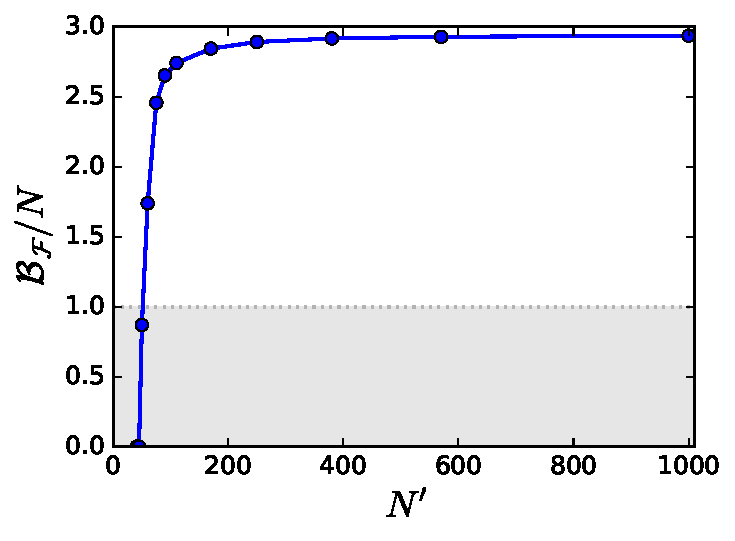
\includegraphics[scale=.65]{img/LT_dicke_7900_asymp.pdf}
  \caption[Asymptotic behaviour of the bound for increasing size systems for Dicke like experimental data]{Secuence of the evolution of an unpolarized Dicke state of 16 qubits for $\theta=\{i\pi/6\}_{i=0}^4$. Bloch spheres representing the Hirusi distribution of the state, and below PDF of the $J_x$ POVM for each step of the secuence}
  \label{fig:assimpthotic-approach-to-the-bound-from-scaled-dicke}
\end{figure}
we plotted the right-hand side of Eq.~\eqref{eq:lt-definitive-formula-scaling-dicke} as the function of $N'$ divided by $N$.
We can see that $\bound{N'}/N$ is constant or slightly increasing for $N'>400$.
This is a strong evidence that Eq.~\eqref{eq:lt-asymptotic-limit-bound-dicke-symmetric} is valid for relatively large particle numbers.
With this, we arrive at the result for the experimental system
\be
  \label{eq:lt-result-experimental-dicke}
  \frac{\bound{N}(\expect{J_y^2},\expect{J_x^2}=\expect{J_z^2})}{N}\approx 2.94.
\ee
The $\approx$ sign is used referring to the fact that we assume that the inequality in Eq.~\eqref{eq:lt-radial-linearity-dicke-bound} is close to be saturated and that we did sufficient numerics for an increasing system size $N'$ to have a good asymptotic approach to the real value Eq.~\eqref{eq:lt-asymptotic-limit-bound-dicke-symmetric}.

It is instructive to compare the value of Eq.~\eqref{eq:lt-result-experimental-dicke} to the one obtained in Section~\ref{sec:vd-testing-with-experimental-data}, where the same system was characterized base on its metrological usefulness.
Such result implies $\qfif{\rho,J_z}/N\geqslant3.3$ which is somewhat bigger than our recent result as we did not use the knowledge of the fourth moments, only the second moments.
The closeness of the two results is a strong argument for the correctness of our calculations.

\subsection{Scaling for $\qfif{\rho,J_z}$ with $N$}

Recent important works examine the scaling of the quantum Fisher information with the particle number for metrology under the presence of decoherence \cite{Escher2011, Demkowicz-Dobrzanski2012}.
They consider the QFI defined now for the non-unitary, noisy evolution.
They find that for small $N$ it is close to the value obtained by considering coherent dynamics.
Hence, even the Heisenberg scaling, $\mathcal{O}(N^2)$, can be reached.
However, if $N$ is sufficiently large, then, due to the decoherence during the parameter estimation, the QFI scales as $\mathcal{O}(N)$.

We have to stress that the findings of \cite{Escher2011, Demkowicz-Dobrzanski2012} are not applicable to our case.
Our methods estimates the quantum Fisher information assuming a perfect unitary dynamics.
The quantum Fisher information can be smaller that what we expect ideally only due to the imperfect preparation of the state\footnote{
This is also relevant for \cite{Augusiak2015}, where $\qfi=\mathcal{O}(N^2)$ is reached with weakly entangled states.}.
We can even find simple conditions on the state preparation that lead to a Heisenberg scaling.
Based on Eq.~\eqref{eq:lt-ghz-legendre-solution}, if we could realize quantum states $\rho_N$ such that $F_{\text{GHZ}}(\rho_N)\geqslant0.5+\epsilon$ for $N\rightarrow\infty$ for some $\epsilon>0$, then we would reach $\bound{\mathcal{F}}(F_{\text{GHZ}}) = \mathcal{O}(N^2)$.
Strong numerical evidence suggest that a similar relation holds for fidelity $F_{\text{Dicke}}$ and $\bound{\mathcal{F}}(F_{\text{GHZ}})$, see Section~\ref{sec:lt-bound-dicke-states}.
[TD: Decide if remove the following sentence. It is very strong]
From another point of view, our method can estimate $\qfif{\rho,J_z}$ for large particle numbers, while a direct measurement of the metrological sensitivity considerably underestimates it.
